\section{Introduction}
\label{sec:intro}

Active automata learning aims to construct black-box state diagram models of software and hardware systems
by providing inputs and observing outputs.
In 1987, Angluin \cite{Ang87} published a seminal paper in which she showed that finite automata can be learned using so-called 
\emph{membership queries} and \emph{equivalence queries}.
Many (if not most) efficient active learning algorithms used
today are designed following Angluin's approach of a \emph{minimally adequate teacher (MAT)}.
In this approach, learning is viewed as a game in which a learner has to infer the behavior of
an unknown state diagram by asking queries to a teacher.
Following pioneering work by \cite{Ang87,PeVaYa02,Hagerer2002,RaMeSM2009,IsHoSt2015},
active automata learning is emerging as an effective bug finding technique.
Using active automata learning, for instance, standard violations have been found in many implementations of
major network and security protocols such as TLS \cite{dRP15}, TCP \cite{FJV14,FJV16,FH17} and SSH \cite{FiterauEtAl17}.

Timing often plays a crucial role in these applications.
A TCP implementation, for instance, may retransmit packets if they are not acknowledged within
a specified time. Also, a timeout may occur if the implementation does not receive an acknowledgement
after a number of retransmissions, or if it remains in certain states too long.
Timing behavior cannot be captured using existing learning tools, which only support learning of deterministic
Mealy machines and related untimed models.
In the case of TCP, previous work only succeeded to learn Mealy machine models by having the network adaptor 
ignore all retransmissions, and by completing learning queries before the occurrence of certain timeouts \cite{FJV16}.
All timing issues had to be artificially suppressed.

There has been some work on algorithms for learning timed systems, e.g., \cite{GrinchteinJL10,MensM15,CCF16}.
The modeling frameworks of \cite{MensM15,CCF16} are very restrictive however: the symbolic automata of \cite{MensM15}
are finite state, which means that timeouts can not be modeled, whereas the time delay Mealy machines of
\cite{CCF16} only have a single timer, which is reset on every transition.
In contrast, the event recording automata studied by \cite{GrinchteinJL10} appear to have too many degrees of freedom,
leading to a complicated learning algorithm with a complexity that is prohibitively high.
For learning, we would like to have a class of models where the occurrence of timing-dependent behavior
is determined by previous behavior, that is, fewer degrees of freedom than what is supported by event-recording automata.

We therefore decided to pursue a different approach. We explore tractable extensions of untimed automata models that appear to
be sufficiently expressive to describe the real-time behavior of network protocols such as TLS, TCP and SSH, and other
applications of automata learning like those described in \cite{Vaa17}.
%
Our work is inspired by the results of \cite{CCF16} on time delay Mealy machines.
We introduce the class of Mealy machines with timers (MMTs) that 
is able to model the timing behavior of a wide variety of communication protocols.
MMTs can be viewed as a formalization of the finite state models with countdown timers that are used in the textbook of
Kurose and Ross \cite{KR13} to explain transport layer protocols.
Figure~\ref{fig:abp} presents an MMT model of the sender from 
the alternating-bit protocol, adapted from \cite[Figure 3.15]{KR13}.
\begin{figure}[h]
\centering
\ifshort
\vspace{-2 em}
\fi
\begin{tikzpicture}[->,>=stealth',shorten >=1pt,auto,node distance=2.3cm,main node/.style={circle,draw,font=\sffamily\large\bfseries}]
  \node[initial, state] (1) {$q_0$};
  \node[state] (2) [right of=1] {$q_1$};
  \node[state] (3) [below of=2] {$q_2$};
  \node[state] (4) [below of=1] {$q_3$};

  \path[every node/.style={font=\sffamily\scriptsize}]
    (1) edge [text width=1.5cm] node {$\mathit{in}/\mathit{send0}$ \\ $x := 3$} (2)
    (2) edge [text width=1.5cm] node {$\mathit{ack0}/\Lambda$ \\ $\mathit{stop}(x)$} (3)
        edge [loop right, text width=1.5cm] node {$\toevent{x}/\mathit{send0}$\\ $x := 3$ } (2)
    (3) edge [text width=1.5cm] node {$\mathit{in}/\mathit{send1}$ \\ $x := 3$} (4)
    (4) edge [text width=1cm] node {$\mathit{ack1}/\Lambda$ \\ $\mathit{stop}(x)$} (1)
        edge [loop left, text width=1.5cm] node {$\toevent{x}/\mathit{send1}$\\ $x := 3$} (4);
\end{tikzpicture}
\caption{MMT model for alternating-bit protocol sender}
\label{fig:abp}
\end{figure}
In the diagram $x :=3$ denotes that a transition starts a timer $x$ with value $3$,
and $\mathit{stop}(x)$ denotes that timer $x$ is stopped.
For readability we have omitted trivial self-loops.
\iflong
$\Lambda$ denotes the absence of an observable output. 

In the model, input $\mathit{in}$ corresponds to a request from the upper layer to transmit data.
Initially, upon receipt of such a request, the sender builds a packet from the data and a sequence number $0$,
sends the packet over the network (output $\mathit{send0}$), and starts the timer with timeout value $3$.
If the sender receives an acknowledgement with the right sequence number $0$ (input $\mathit{ack0}$) 
then it stops the timer and jumps to state $q_2$.
Acknowledgement with the incorrect sequence number (input $\mathit{ack1}$) are ignored.
If no $\mathit{ack0}$ input arrives within $3$ timeunits, a timeout occurs and the same packet is sent again.
The behavior in states $q_2$ and state $q_3$ is analogous to that in states $q_0$ and $q_1$, respectively,
with the roles of $0$ and $1$ swapped.
\fi
The approaches of \cite{MensM15,CCF16} cannot model this protocol.

%The remainder of this article is structured as follows.
In Section 2, we present the definition of MMTs, their timed semantics, and a minimally adequate teacher for MMTs.
Our timed semantics is based on \emph{timed words} that record the timing of inputs and outputs. 
Since we assume that each timeout immediately triggers an observable output, we may observe
the occurrence of a timeout indirectly. However, we cannot observe which timer times out.
In a membership query, a learner specifies at which specific times input events occur. In response, the teacher
specifies which outputs occur in response to these inputs, as well as the timing of these outputs.
Via an equivalence query, the learner asks whether an hypothesis MMT that it has constructed accepts the same timed words
as the (unknown) MMT of the teacher. The teacher answers `yes' if this is the case and `no' otherwise.
In case of a `no' answer, a timed word is provided that illustrates why the hypothesis is incorrect.

In Section 3, we present a surprising result, namely that under certain mild restrictions our timed semantics for MMTs
is the same as an untimed semantics in which behaviors record when and how timers are set and when they expire.
Intuitively, causality of timeouts can be inferred in the timed semantics since a slight change in the timing of an input event leads to a corresponding change in the timing of any timeout that it induces.

The result of Section 3 suggests an architecture for our learning algorithm that is shown in Figure~\ref{architecture}.
The idea is to define an alternative (and simpler) MAT framework in which the learner uses membership queries (MQ) and equivalence queries (EQ)
to obtain information about the untimed behaviors of an MMT.
An adapter then implements each untimed membership query via a series of timed membership queries for the timed teacher,
and each untimed equivalence query via a timed equivalence query.
\begin{figure}[h]
\begin{center}
 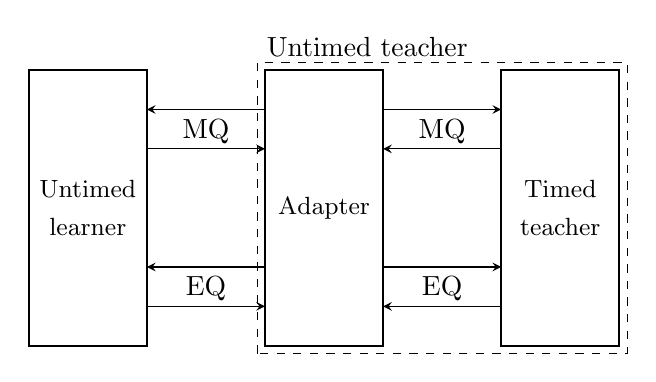
\begin{tikzpicture}[>=stealth]
 \draw [dashed] (-0.1,-0.1) rectangle (4.6,3.6);
 \node [above,right] at (-0.1,3.8) {Untimed teacher};
            \draw [thick] (0,0) rectangle (1.5,3.5) node[midway] {\small Adapter};
            \draw [thick] (3,0) rectangle (4.5,3.5) node[midway,above] {\small Timed};
            \draw [thick] (3,0) rectangle (4.5,3.5) node[midway,below] {\small teacher};
            \draw [->] (1.5,3) -- (3,3) node[midway,below] {MQ};
            \draw [<-] (1.5,2.5) -- (3,2.5);
            \draw [->] (1.5,1) -- (3,1) node[midway,below] {EQ};
            \draw [<-] (1.5,0.5) -- (3,0.5);
            \draw [->] (0,3) -- (-1.5,3) node[midway,below] {MQ};
            \draw [<-] (0,2.5) -- (-1.5,2.5);
            \draw [->] (0,1) -- (-1.5,1) node[midway,below] {EQ};
            \draw [<-] (0,0.5) -- (-1.5,0.5);
            \draw [thick] (-3,0) rectangle (-1.5,3.5) node[midway,above] {\small Untimed};
            \draw [thick] (-3,0) rectangle (-1.5,3.5) node[midway,below] {\small learner};
        \end{tikzpicture}
\end{center}
\caption{Learning architecture}
\label{architecture}
\end{figure}
Section~\ref{algorithm} describes the untimed MAT framework for MMTs and the adapter that implements an untimed teacher using
a timed teacher.

Section~\ref{sec:approx} then presents an algorithm for the untimed MMT learner, based on a Myhill-Nerode theorem for the untimed semantics. 
Section~\ref{conclusions} contains some concluding remarks and lists topics for future research.
\ifshort
A full version of this article including proofs is available at \url{http://www.sws.cs.ru.nl/publications/papers/fvaan/MMT}.
\fi

